\begin{figure}[H]
\centering
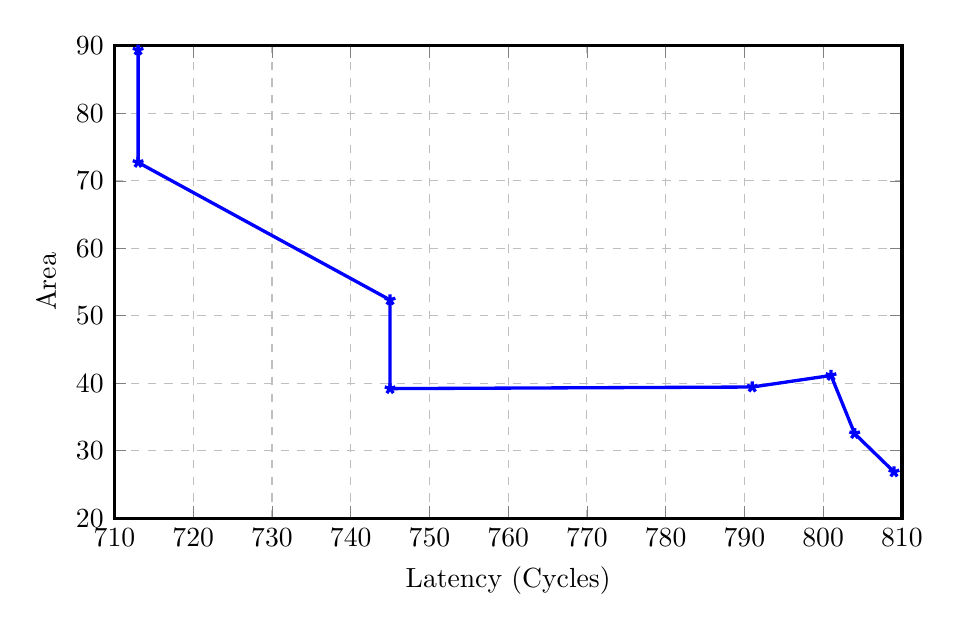
\begin{tikzpicture}
\begin{axis}[
scale only axis,
height=6cm,
width=10cm,
    xlabel={Latency (Cycles)},
    ylabel={Area},
    xmin=710, xmax=810,
    ymin=20, ymax=90,
    xtick={710,720,730,740,750,760,770,780,790,800,810},
    ytick={20,30,40,50,60,70,80,90},
    legend pos=north east,
    ymajorgrids=true,
    xmajorgrids=true,
    grid style=dashed,
    very thick
]
\addplot[
    color=blue,
    mark=star,
   % smooth
    ]
    coordinates {
    (713,89.37)(713,72.72)(745,52.345)(745,39.204)(791,39.441)(801,41.154)(804,32.54)(809,26.8625)
    };
\end{axis}
\end{tikzpicture}
\caption{Area Vs. Latency Curve for 16-Point FFT Implementation}
\label{plot_16fft}
\end{figure}